This section describes the distributions used in the MH and PF algorithms as well as experiments used for validation.

\subsection{Distributions and Parameters}
\label{distribution}
In order to use Bayesian algorithms, one must designate a prior which generally captures the structure of the true prior distribution. As more data becomes available, the prior has less effect on the MAP solution, so for data rich applications, the exact formulation of the prior is not as important. Since the weight and dimensions of each human operator will be different, we non-dimensionalize the distribution by considering the distribution over mass fraction (i.e. $\frac{m_{ij}}{\sum m_{ij}}$) and the distance of the center of mass relative to the link length, $\rho_{ij}$. 

In the experiments section, the prior over the masses and center of masses is modeled as a Gaussian with truncated tails and hard constraints that the body masses are symmetric and that the mass sums to one. 
The mean and standard deviation over the masses $m_{ij}$ and center of masses $\rho_{ij}$ are derived primarily from \cite{jensen1989changes,armstrong1988anthropometry} and are listed in Table \ref{table:prior}. 
The tails are truncated such that no body part has negative mass and such that the center of mass is contained within the link modeling the body part.
Additionally, we constrain the distribution such that left-right symmetry is maintained and such that the masses sum to one. Mathematically,
\begin{equation}
p(\theta) \propto
\left\{
  \begin{array}{lc}
    	0& : \sum m_{ij} \neq 1 \\
	0& : \exists m_{ij} < 0 \\
	0& : \exists \rho_{ij} < 0 \\
	0& : \exists \rho_{ij} > 1 \\
	0& : \text{Not symmetric}  \\
    	\mathcal{N}(\mu_\theta,\Sigma_\theta) & : \text{otherwise}
    
  \end{array}
\right.
\end{equation}
where the mean values and variances are given in Table \ref{table:prior}.
The measurement likelihood function is modeled as a Gaussian with mean given by the right hand side of \eqref{eq:comSum}, with variance $\omega^2 = 100^2\text{mm}^2$,
\begin{equation}
p(y \mid \theta, r) = \mathcal{N}(\sum_{(i,j)\in\mathcal{L}} m_{ij} r_i + m_{ij}\rho_{ij}(r_j - r_i), 100^2)
\end{equation}

\begin{table}
\caption{Parameters for Prior Distribution}
\label{table:prior}
\begin{center}
\begin{tabular}{|c|c|c|}
\hline
           & m (mean, variance) & $\rho$ (mean, variance) \\
\hline
 Head+Neck & $(0.0775, 0.05^2)$ & $(0.5344, 0.05^2)$ \\
\hline
 Upper Torso & $(0.1284, 0.05^2)$ & $(0.5529, 0.05^2) $\\
\hline
 Lower Torso & $(0.7233, 0.05^2)$ & $(0.4903, 0.05^2) $\\
\hline
 Upper Arm & $(0.0401, 0.05^2)$ & $(0.5503, 0.05^2)$ \\
\hline
 Lower Arm+Hand & $(0.0291, 0.05^2)$ & $(0.7115, 0.05^2)$ \\
\hline
 Upper Leg & $(0.0987, 0.05^2)$ & $(0.4482, 0.05^2) $\\
\hline
 Lower Leg+Foot & $(0.0364, 0.05^2)$ & $(0.5797, 0.05^2)$ \\
\hline
\end{tabular}
\end{center}
\end{table}

%\begin{table*}
%\caption{Parameters for Prior Distribution}
%\label{table:prior}
%\begin{center}
%\begin{tabular}{|c|c|c|c|c|c|c|c|}
%\hline
% &Head+Neck & Upper Torso & Lower Torso & Upper Arm & Lower Arm+Hand & Upper Leg & Lower Leg+Foot\\
%\hline
% $m$ Fraction Mean &0.0775 & 0.1284 & 0.2733 & 0.0401 & 0.0291 & 0.0987& 0.0364 \\
%\hline
% $m$ Fraction Variance & $0.05^2$ & $0.05^2$ & $0.05^2$ & $0.05^2$ & $0.05^2$ & $0.05^2$ & $0.05^2$\\
%\hline
% $\rho$ Mean &0.5433& 0.5529 & 0.4903 & 0.5503 & 0.7115 & 0.4482 & 0.5797 \\
%\hline
% $\rho$ Variance & $0.05^2$ & $0.05^2$ & $0.05^2$ & $0.05^2$ & $0.05^2$ & $0.05^2$ & $0.05^2$\\
%\hline
%\end{tabular}
%\end{center}
%\end{table*}
%\begin{tabularx}{\textwidth}
%\caption{Parameters for Prior Distristribution}
%\label{table:prior}
 % \toprule
%  xx&1&2&3\\
%  xx&1&2&3\\
%  \bottomrule
%\end{tabularx}

In the experiments, the following parameters were used for the MH and PF algorithms: $\sigma_{PF} = 0.005$, $\alpha_{PF} = 0.01$, $K=100$, and $\sigma_{MH} = 0.01$.

\subsection{Experiments}
\label{experiments}
In order to validate the methods for parameter identification and center of mass prediction, five subjects were tested. 
Each subject performed in two trials. In each trial, the subject moved slowly and demonstrated a variety of different poses for approximately two minutes. 
The first of these trials was used as a training dataset by the algorithms to estimate the mass distribution, and the second data trial was used as a validation, or test, dataset. 
In addition to testing the MH and PF algorithms, we also compare our methods to the SECS model of \cite{gonzalez2012estimation}, which does not estimate the mass distribution but estimates regression coefficients that can be used to predict the center of mass from angle positions.

We compare the predicted center of mass to that measured by the Wii balance board on the second \emph{testing dataset}, which is different from the first dataset used to train the algorithms. For testing CoM prediction, the MH and PF MAP estimates are plugged into $\theta$ of \eqref{eq:comSum}. 
There is no way to directly measure the inertial parameters of the human, so this paper simply compares the output of these algorithms to the prior distribution. Further work will focus on other validation methods.

A Kinect camera estimates the pose of the human using the built-in skeleton detection algorithm, with sampling frequency approximately 30~Hz. The wii balance board records the center of pressure, which is assumed to be close to the center of mass, in the horizontal place at approximately 60~Hz. 
Both Kinect and balance board measurements are first filtered using a median filter and then a sliding average filter. The median filter considers the nearest 7 measurements and is used to filter outliers that sporadically occur when the Kinect skeleton detection algorithm loses track of the skeleton. The sliding window filter has the purpose of both filtering noise as well as accounting for different sensor sampling rates. In particular, the sliding average filter interpolates the observation value by taking a weighted moving average of all observations within a $0.1$~s window. %using a window shape $\frac{1}{1+\beta(\Delta T)^2}$.
%: $\hat y = \sum \frac{1}{1+(\Delta T)^2} y_i$


Table \ref{table:RMSE} compares the mean absolute error (MAE) predicting the center of mass for each person. Figure \ref{fig:com1} shows example CoM trajectories and predictions for the test trials. Lastly, table \ref{table:massdist} shows the inertial parameter estimates compared with the initial prior estimates for one subject.
\begin{table}
\caption{CoM Prediction MAE (mm)}
\label{table:RMSE}
\begin{center}
\begin{tabular}{|c|c|c|c|c|c|}
\hline
 & Subject 1 & Subject 2 & Subject 3 & Subject 4 & Subject 5\\
\hline
MH & 28.87   & 27.88 & 30.59 & 16.56 & 22.13\\
\hline
PF & 27.68 1 & 27.43 & 30.69 & 18.79 & 23.44\\
\hline
SESC & 60.06 & 65.92 & 43.49 & 42.52 &  59.9\\
\hline
\end{tabular}
\end{center}
\end{table}








\begin{table*}[t]
\caption{Mass Distribution for Subject 1-5. Parameters listed in tuples ($m$ fraction, $\rho$)}
\label{table:massdist}
\begin{center}
\begin{tabular}{|c|c|c|c|c|c|c|c|}
\hline
 &Head+Neck & Upper Torso & Lower Torso & Upper Arm & Lower Arm+Hand & Upper Leg & Lower Leg+Foot\\
\hline
\hline
 Prior Mean &(0.0775,0.5433) & (0.1284,0.5529) & (0.2733,0.4903) & (0.0401,0.5503) & (0.0291,0.7115) & (0.0987,0.4482) & (0.0364,0.5797) \\
\hline
  \multicolumn{8}{|c|}{Subject 1} \\
\hline
 MH Estimate &(0.0494,0.5408) & (0.1193,0.5216) & (0.4394,0.5523) & (0.0149,0.5704) & (0.0107,0.7185) & (0.0891,0.3708) & (0.0812,0.6379) \\
\hline
 PF Estimate & (0.0349,0.5473) & (0.1436,0.5288) & (0.4051,0.5231) & (0.0218,0.5505) & (0.0095,0.7140) &  (0.1050,0.4064) & (0.0720,0.6088) \\
\hline
  \multicolumn{8}{|c|}{Subject 2} \\
\hline
 MH Estimate & (0.0140,0.5119) & (0.1142,0.5441) & (0.3929,0.5773) & (0.1077,0.5245) & (0.0099,0.7074) & (0.1120,0.4275) & (0.0099,0.6768) \\
\hline
 PF Estimate & (0.0105,0.5382) & (0.1446,0.5503) & (0.3340,0.5151) & (0.1015,0.5759) & (0.0098,0.7066) & (0.1003,0.4364) & (0.0439,0.6333) \\
\hline
  \multicolumn{8}{|c|}{Subject 3} \\
\hline
 MH Estimate & (0.0134,0.4719) & (0.3422,0.4982) & (0.3965,0.4678) & (0.0104,0.5116) & (0.0104,0.6882) & (0.0240,0.4320) & (0.0791,0.6881) \\
\hline
 PF Estimate & (0.0447,0.5175) & (0.2877,0.5700) & (0.3630,0.4720) & (0.0097,0.5552) & (0.0098,0.7222) & (0.0713,0.4346) & (0.0616,0.6032) \\
\hline
  \multicolumn{8}{|c|}{Subject 4} \\
\hline
 MH Estimate & (0.0134,0.4697) & (0.3422,0.5451) & (0.3965,0.6114) & (0.0102,0.5240) & (0.0102,0.6835) & (0.0460,0.4088) & (0.0843,0.6842) \\
\hline
 PF Estimate & (0.1046,0.5346) & (0.1953,0.5393) & (0.3384,0.4792) & (0.0103,0.5522) & (0.0101,0.7028) & (0.0876,0.4313) & (0.0729,0.5962) \\
\hline
  \multicolumn{8}{|c|}{Subject 5} \\
\hline
 MH Estimate & (0.1943,0.5992) & (0.0255,0.4678) & (0.4212,0.5487) & (0.0106,0.5193) & (0.0106,0.6784) & (0.0360,0.4140) & (0.1223,0.6899) \\
\hline
 PF Estimate & (0.1219,0.5746) & (0.1332,0.5386) & (0.3436,0.5075) & (0.0098,0.5506) & (0.0173,0.7232) & (0.0581,0.4261) & (0.1154,0.6448) \\
\hline
\end{tabular}
\end{center}
\end{table*}














%\begin{table*}[h]
%\caption{Mass Distristribution for Subject 1-5}
%\label{table:massdist}
%\begin{center}
%\begin{tabular}{|c|c|c|c|c|c|c|c|}
%\hline
% &Head+Neck & Upper Torso & Lower Torso & Upper Arm & Lower Arm+Hand & Upper Leg & Lower Leg+Foot\\
%\hline
% $m$ Fraction Prior Mean &0.0775 & 0.1284 & 0.2733 & 0.0401 & 0.0291 & 0.0987& 0.0364 \\
%\hline
% $\rho$ Prior Mean &0.5433& 0.5529 & 0.4903 & 0.5503 & 0.7115 & 0.4482 & 0.5797 \\
%\hline
%\hline
% Subject 1& & & & & &  & \\
%\hline
% $m$ Fraction MH Estimate &0.0494 & 0.1193 & 0.4394 & 0.0149 & 0.0107 & 0.0891& 0.0812 \\
%\hline
% $m$ Fraction PF Estimate & 0.0349 & 0.1436 & 0.4051 & 0.0218 & 0.0095 &  0.1050 & 0.0720 \\
%\hline
%
% $\rho$ MH Estimate &0.5408& 0.5216 & 0.5523 & 0.5704 & 0.7185 & 0.3708 & 0.6379 \\
%\hline
% $\rho$ PF Estimate &0.5473 & 0.5288 & 0.5231 & 0.5505 & 0.7140 & 0.4064 & 0.6088 \\
%
%
%\hline
%\hline
% Subject 2& & & & & &  & \\
%\hline
% $m$ Fraction MH Estimate &0.0140 & 0.1142  & 0.3929 & 0.1077 & 0.0099 & 0.1120 & 0.0099 \\
%\hline
% $m$ Fraction PF Estimate & 0.0105 & 0.1446 & 0.3340 & 0.1015 & 0.0098 &  0.1003 & 0.0439 \\
%\hline
% $\rho$ MH Estimate &0.5119& 0.5441 & 0.5773 & 0.5245 & 0.7074 & 0.4375 & 0.6768 \\
%\hline
% $\rho$ PF Estimate &0.5382 & 0.5503 & 0.5151 & 0.5759 & 0.7066 & 0.4364 & 0.6333 \\ 
%
%\hline
%\hline
% Subject 3& & & & & &  & \\
%\hline
% $m$ Fraction MH Estimate &0.0134 & 0.3422  & 0.3965 & 0.0104 & 0.0104 & 0.0240 & 0.0791 \\
%\hline
% $m$ Fraction PF Estimate & 0.0447 & 0.2877 & 0.3630 & 0.0097 & 0.0098 &  0.0713 & 0.0616 \\
%\hline
% $\rho$ MH Estimate &0.4719& 0.4982 & 0.4678 & 0.5116 & 0.6882 & 0.4320 & 0.6881 \\
%\hline
% $\rho$ PF Estimate &0.5175 & 0.5700 & 0.4720 & 0.5552 & 0.7222 & 0.4346 & 0.6032 \\
%
%\hline
%\hline
% Subject 4& & & & & &  & \\
%\hline
% &Head+Neck & Upper Torso & Lower Torso & Upper Arm & Lower Arm+Hand & Upper Leg & Lower Leg+Foot\\
%\hline
% $m$ Fraction MH Estimate &0.0134 & 0.3422  & 0.3965 & 0.0102 & 0.0102 & 0.0460 & 0.0843 \\
%\hline
% $m$ Fraction PF Estimate & 0.1046 & 0.1953 & 0.3384 & 0.0103 & 0.0101 &  0.0876 & 0.0729 \\
%\hline
% $\rho$ MH Estimate &0.4697& 0.5451 & 0.6114 & 0.5240 & 0.6835 & 0.4088 & 0.6842 \\
%\hline
% $\rho$ PF Estimate &0.5346 & 0.5393 & 0.4792 & 0.5522 & 0.7028 & 0.4313 & 0.5962 \\
%
%\hline
%\hline
% Subject 5& & & & & &  & \\
%\hline
% &Head+Neck & Upper Torso & Lower Torso & Upper Arm & Lower Arm+Hand & Upper Leg & Lower Leg+Foot\\
%\hline
% $m$ Fraction MH Estimate &0.1943 & 0.0255  & 0.4212 & 0.0106 & 0.0106 & 0.0360 & 0.1223 \\
%\hline
% $m$ Fraction PF Estimate & 0.1219 & 0.1332 & 0.3436 & 0.0098 & 0.0173 &  0.0581 & 0.1154 \\
%\hline
% $\rho$ MH Estimate &0.5992& 0.4678 & 0.5487 & 0.5193 & 0.6784 & 0.4140 & 0.6899 \\
%\hline
% $\rho$ PF Estimate &0.5746 & 0.5386 & 0.5075 & 0.5506 & 0.7232 & 0.4261 & 0.6448 \\
%\hline
%\end{tabular}
%\end{center}
%\end{table*}

\begin{figure}
\centering
\vskip -2cm
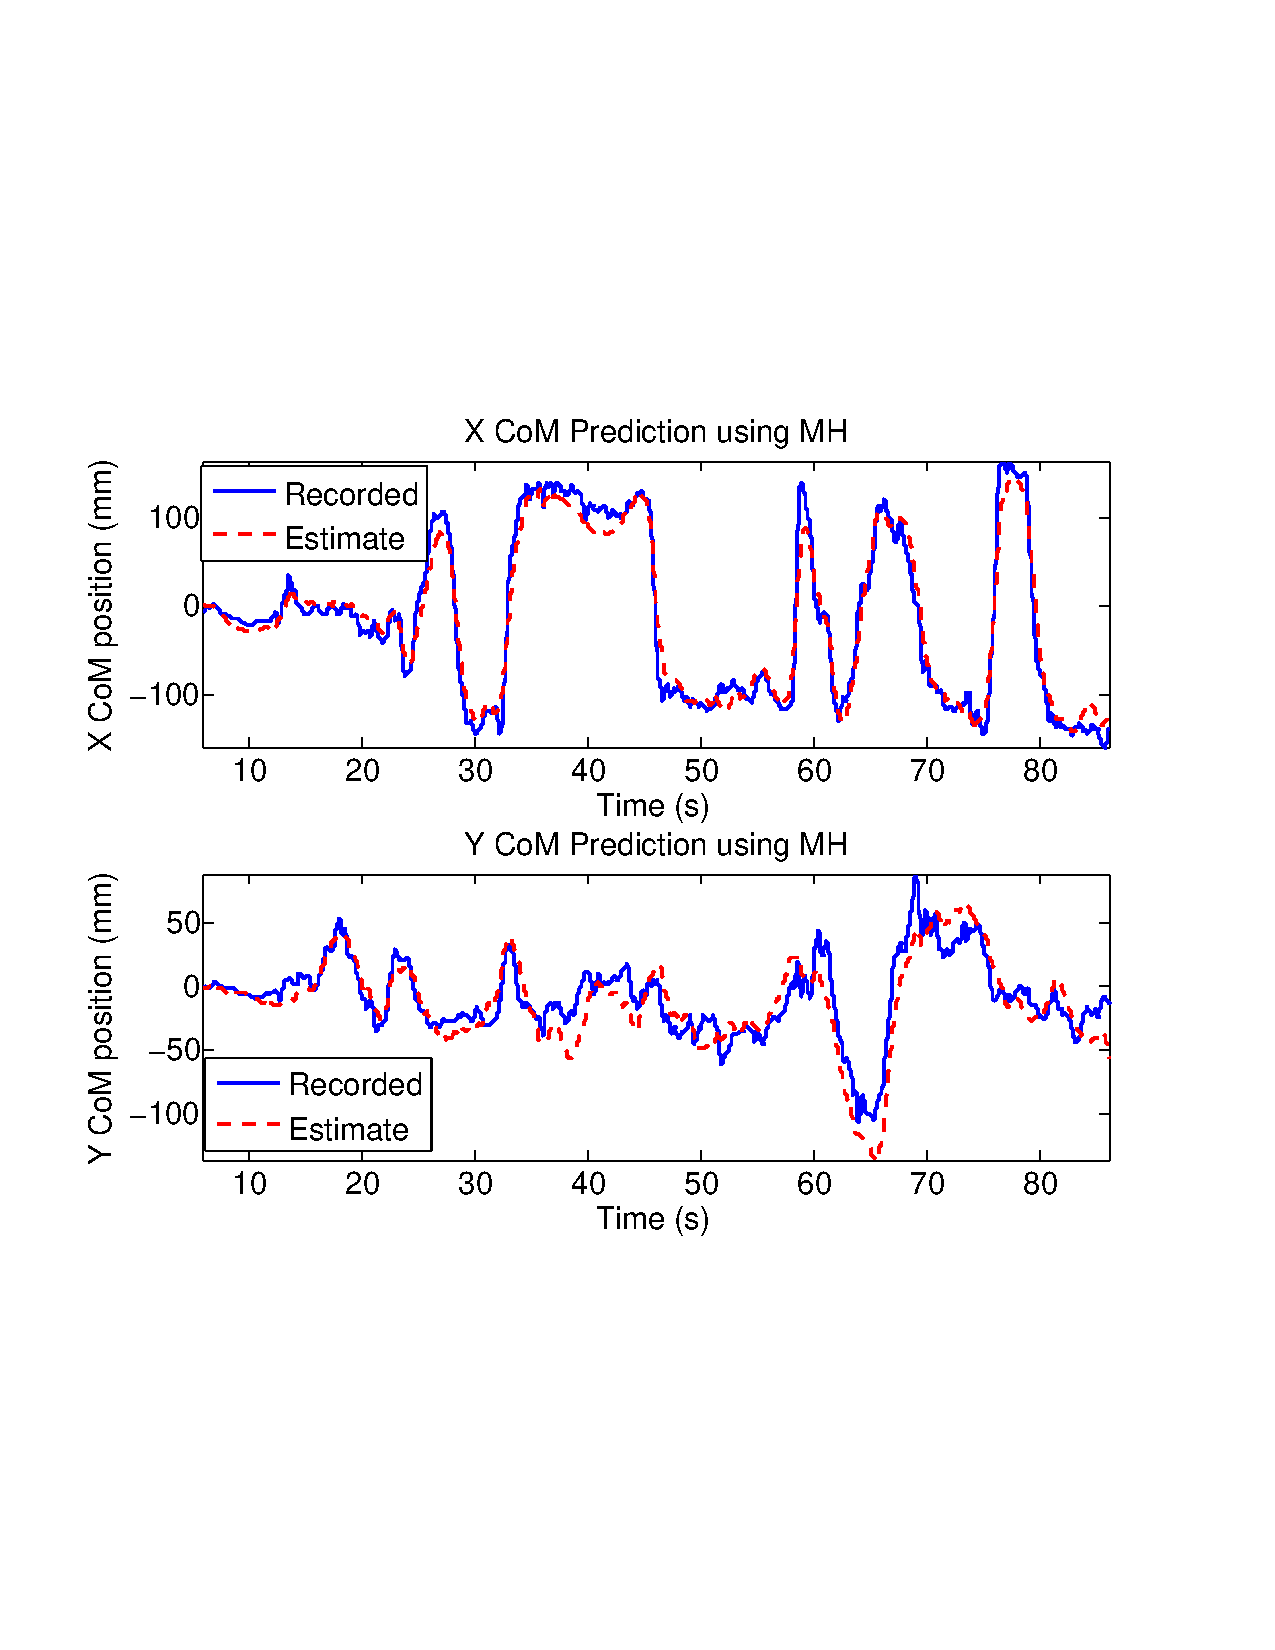
\includegraphics[trim=1cm 6cm 2cm 4cm, clip=true, width=\columnwidth]{figures/MH_Test2.pdf} 
\vskip -0.5cm
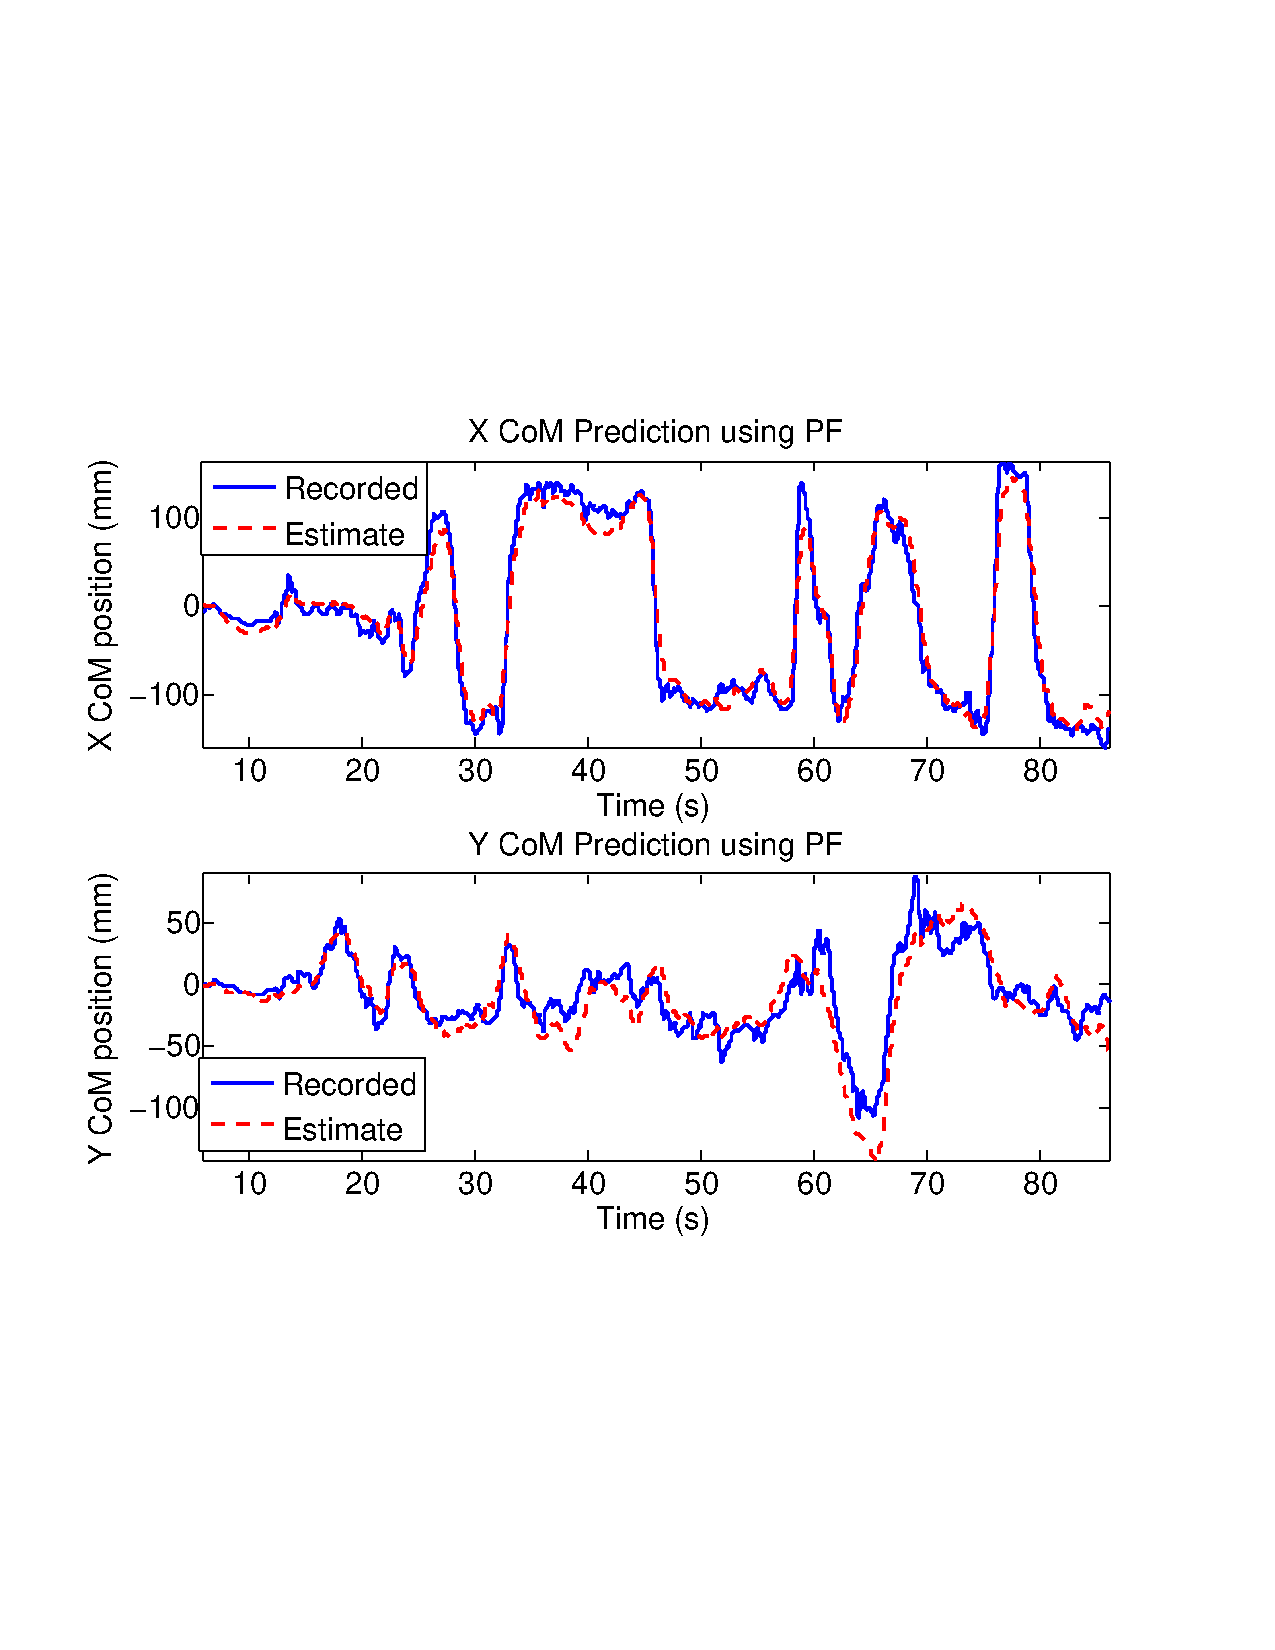
\includegraphics[trim=1cm 6cm 2cm 4cm, clip=true, width=\columnwidth]{figures/PF_Test2.pdf}
\vskip -0.5cm
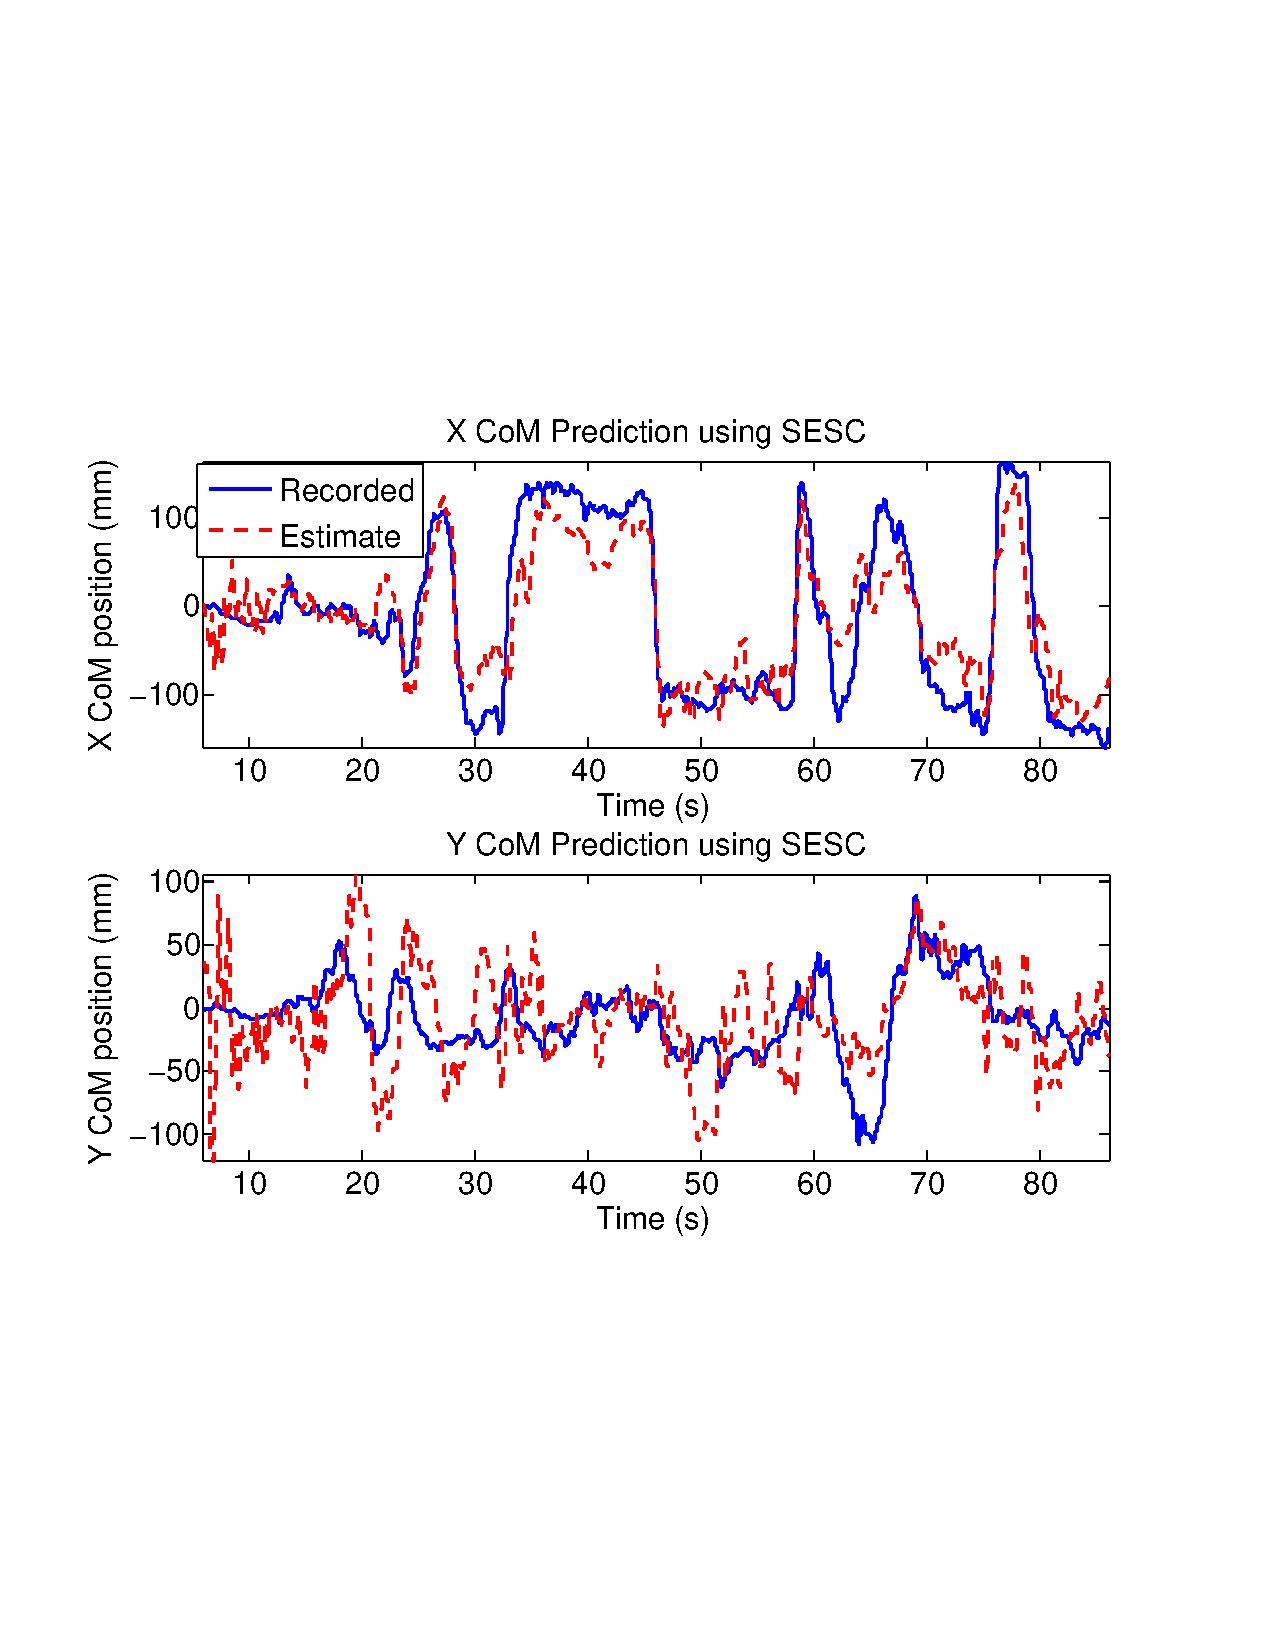
\includegraphics[trim=1cm 6cm 2cm 4cm, clip=true, width=\columnwidth]{figures/SESC_Test2.pdf}  
%   
\caption{CoM prediction using (Top) MH, (Middle) PF, (Bottom) SESC}
\label{fig:com1}
\end{figure}

%\begin{figure*}
%\begin{tabular}{ccc}
%\begin{subfigure}
%  \centering
%    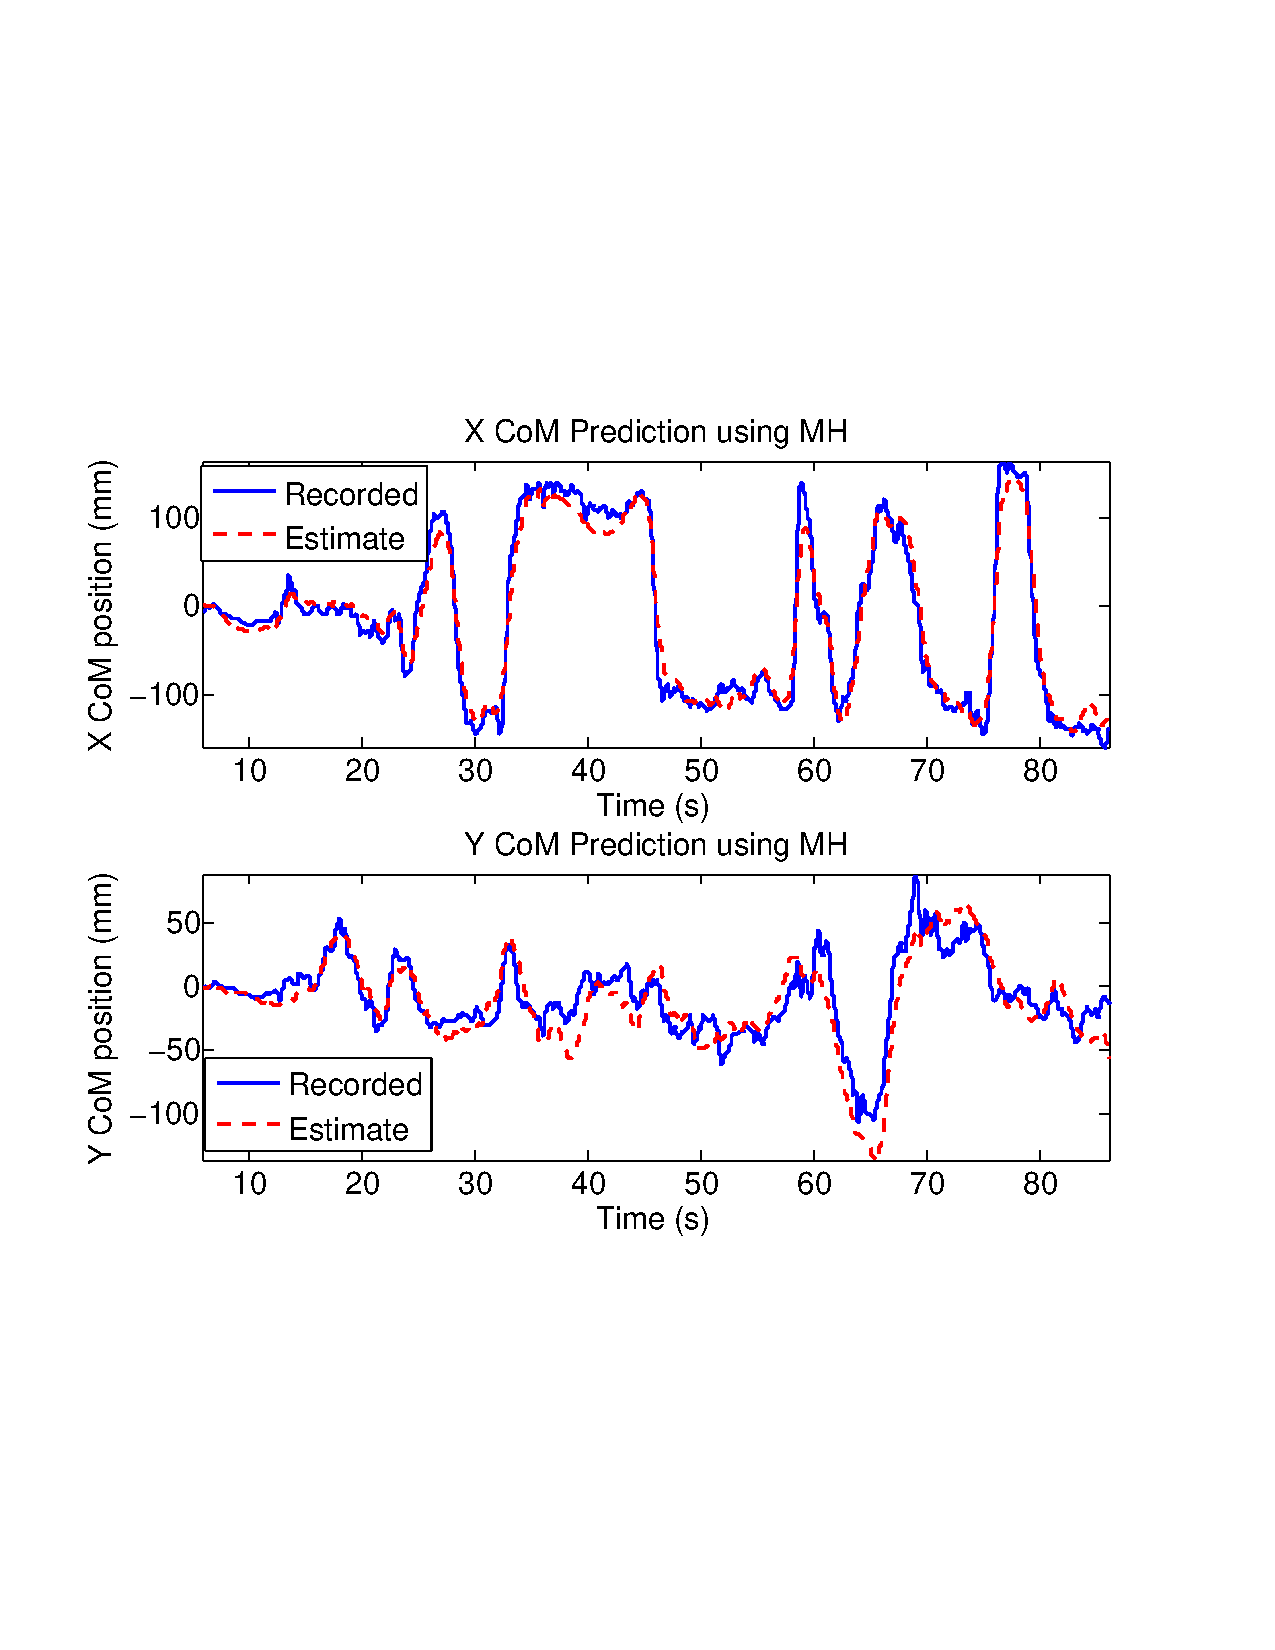
\includegraphics[trim=1cm 6cm 2cm 4cm, clip=true, width=0.6\columnwidth]{figures/MH_Test2.pdf} 
%\end{subfigure} &
%\hspace{-0.3in}
%\begin{subfigure}
%  \centering
%    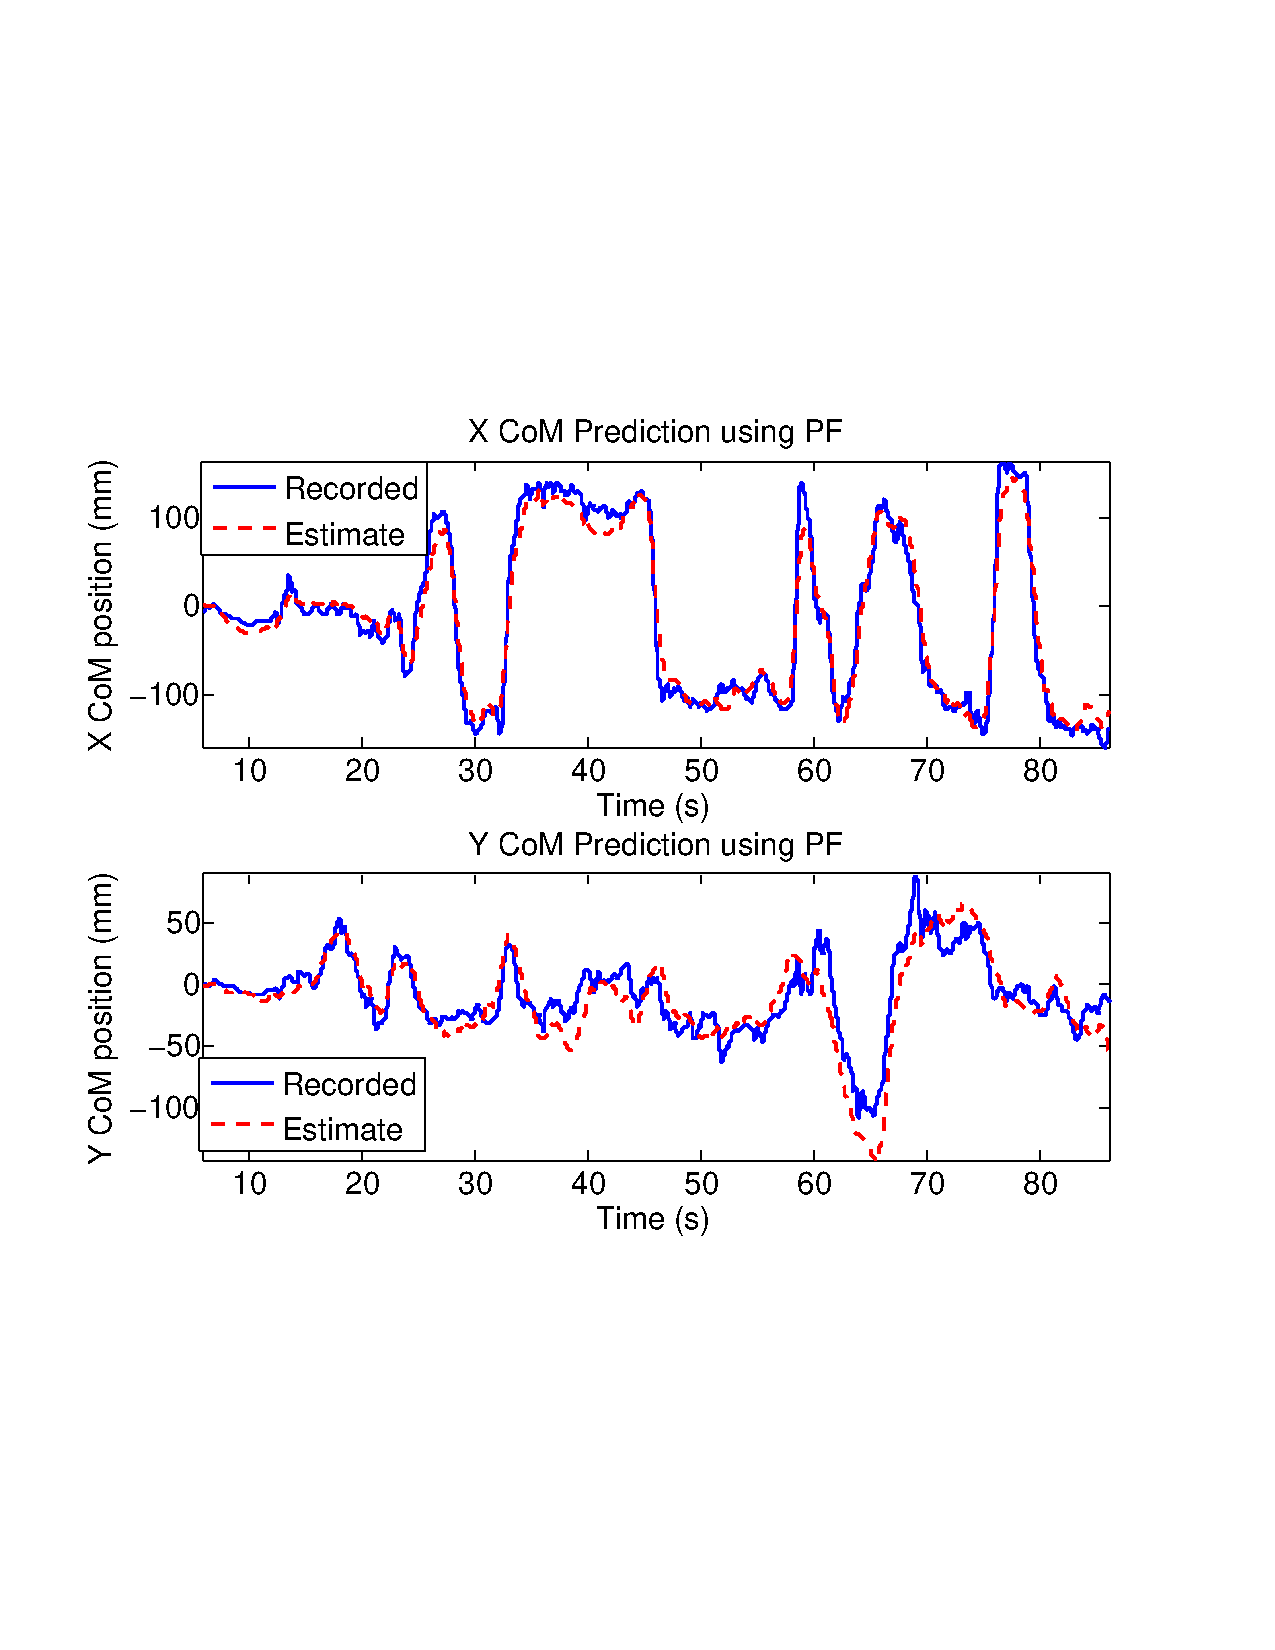
\includegraphics[trim=1cm 6cm 2cm 4cm, clip=true, width=0.6\columnwidth]{figures/PF_Test2.pdf} 
%\end{subfigure} &
%\hspace{-0.3in}
%\begin{subfigure}
%  \centering
%    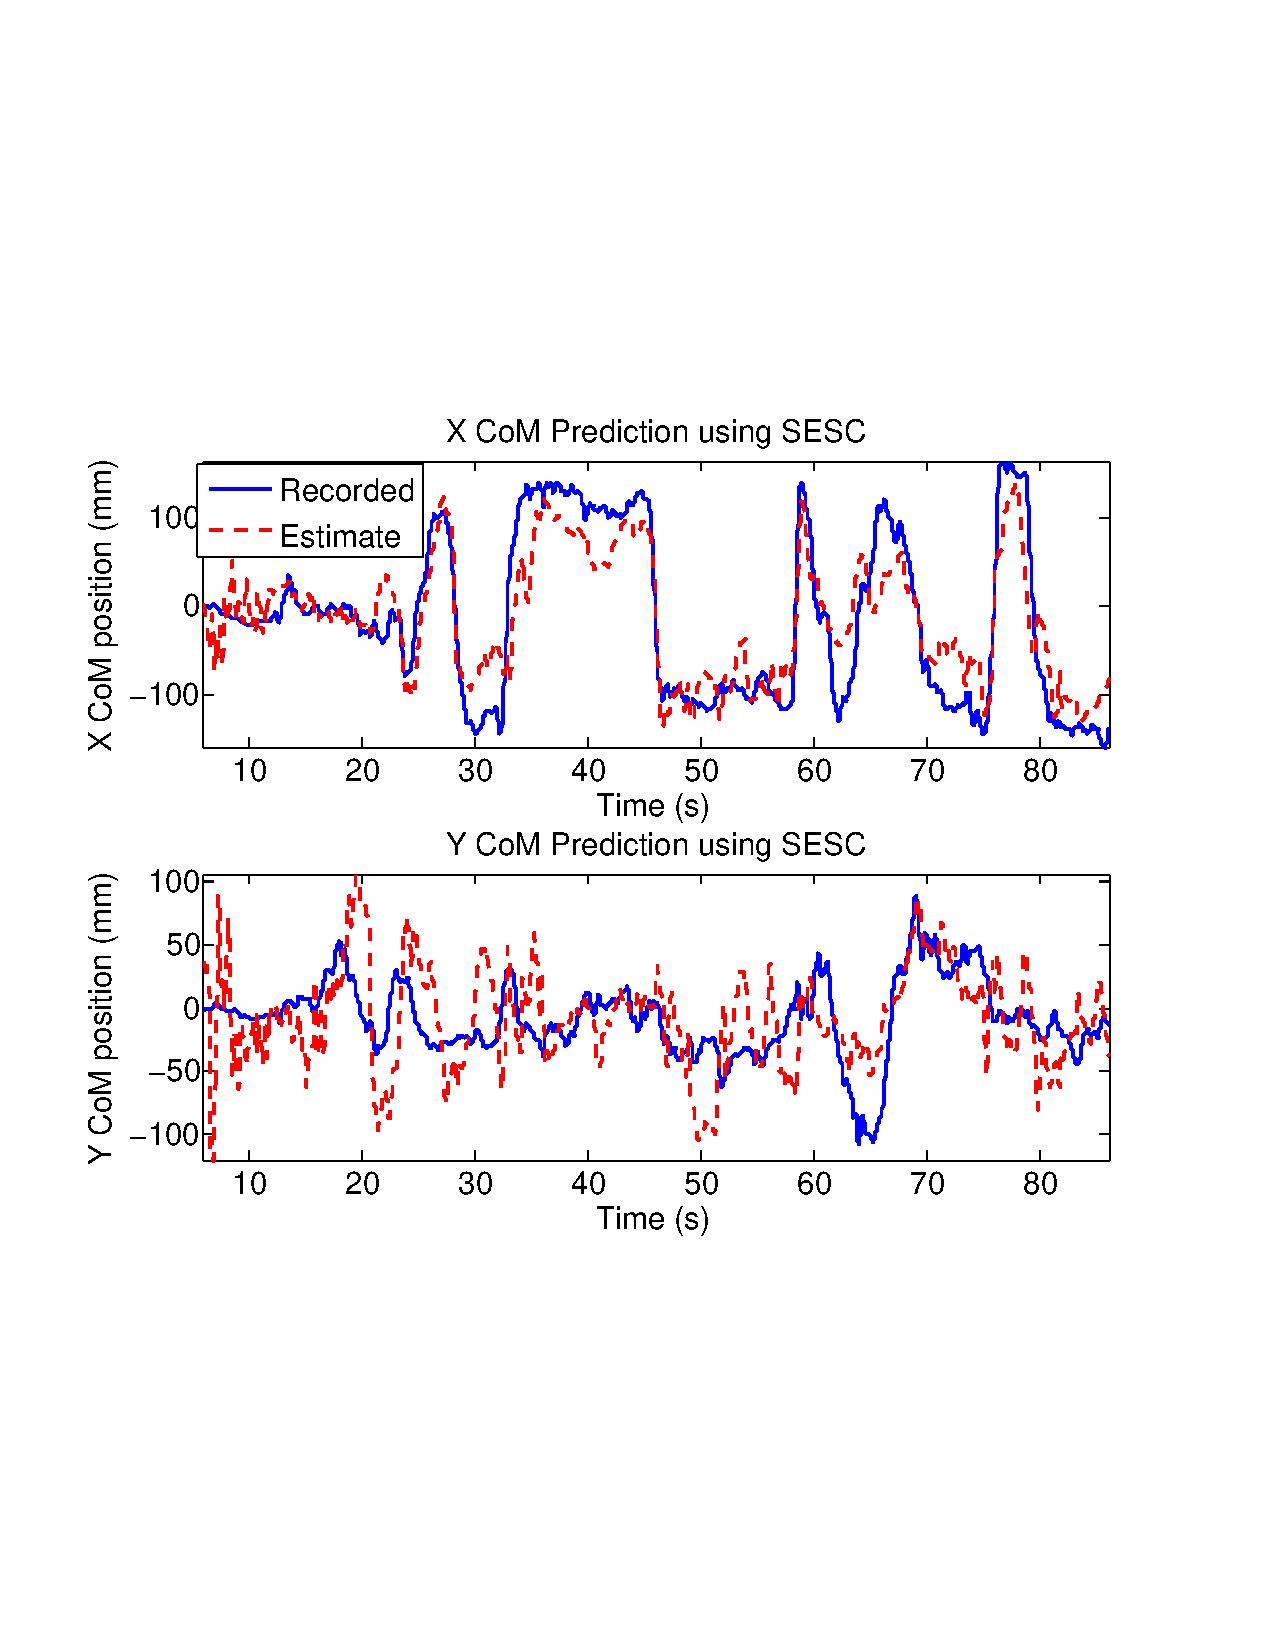
\includegraphics[trim=1cm 6cm 2cm 4cm, clip=true, width=0.6\columnwidth]{figures/SESC_Test2.pdf} 
%\end{subfigure}
%\end{tabular}
%\caption{CoM prediction using (Top) MH, (Middle) PF, (Bottom) SESC}
%\label{fig:pedestrian}
%\end{figure*}
%
%\begin{figure}
%  \centering
%    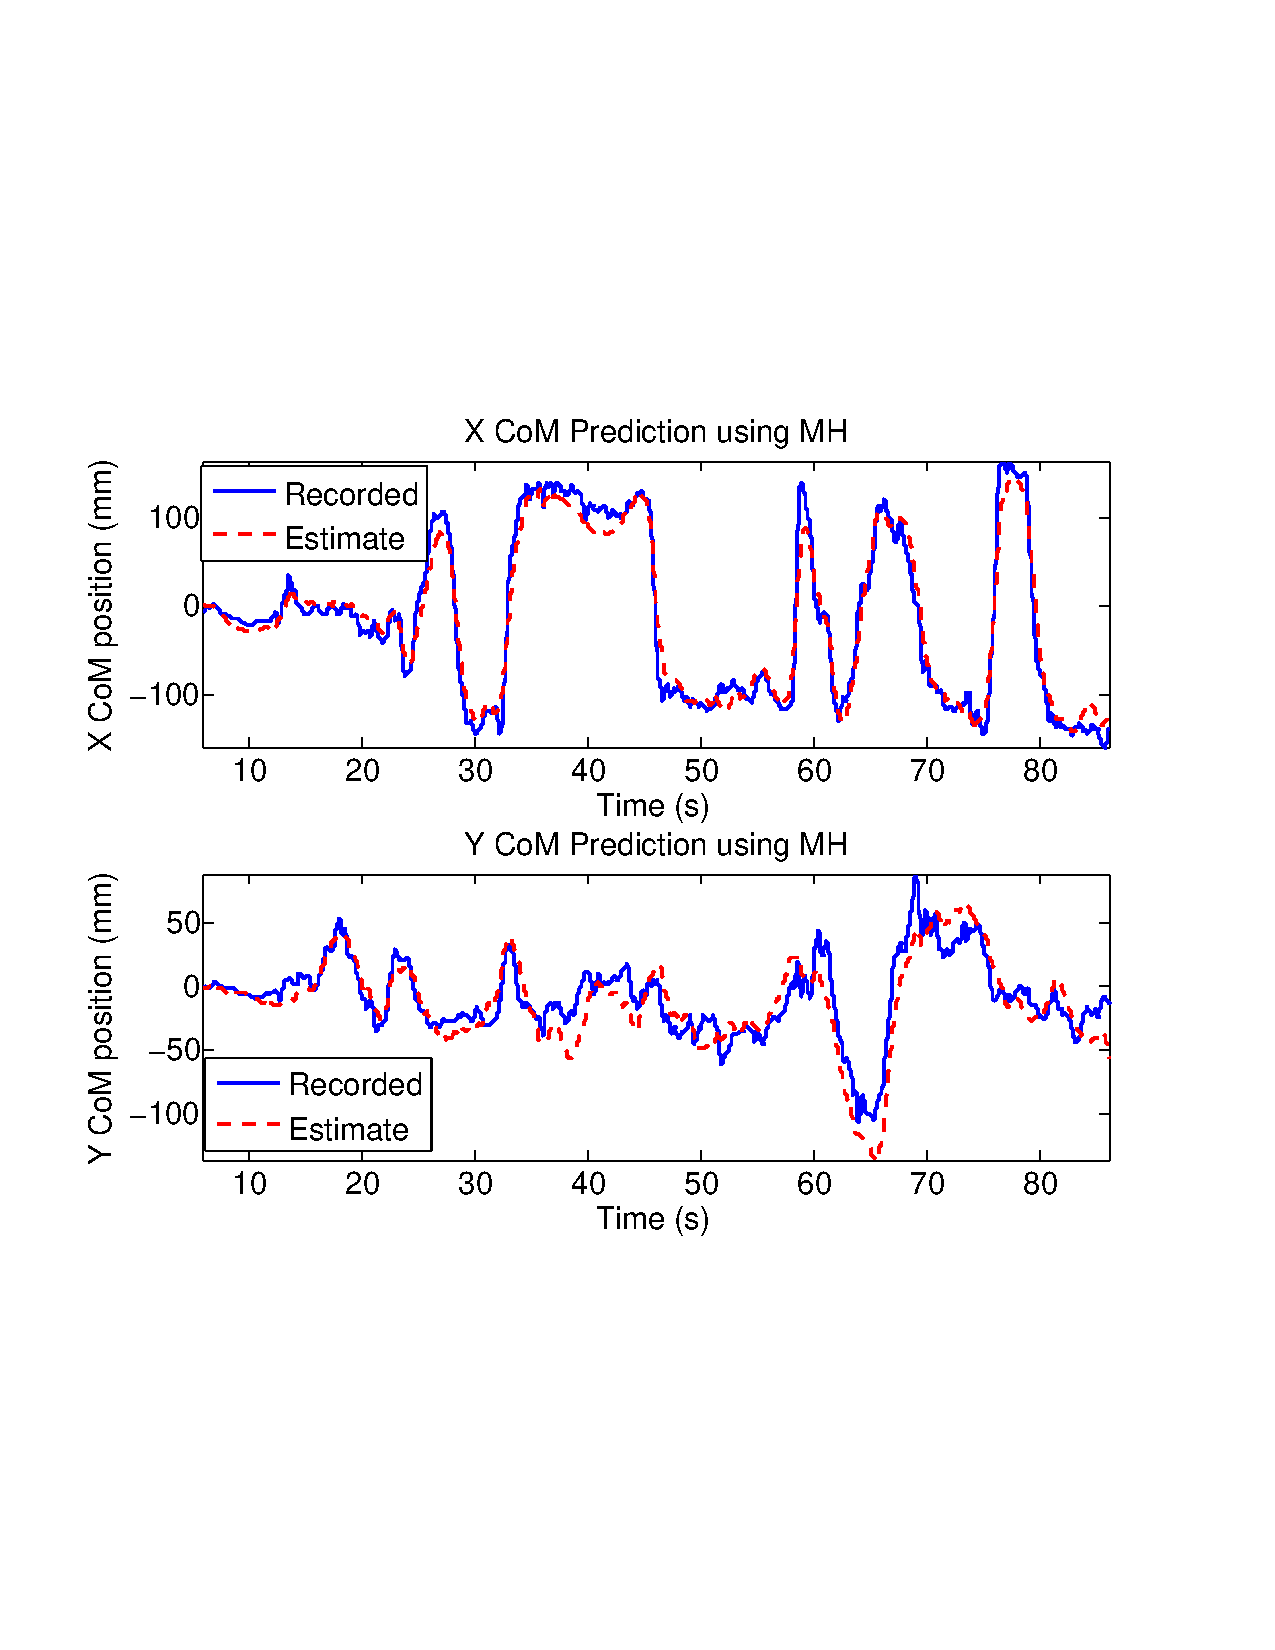
\includegraphics[trim=1cm 6cm 2cm 4cm, clip=true, width=0.9\columnwidth]{figures/MH_Test2.pdf}
%\vspace{-0.15in}
%\caption{CoM prediction using mass distribution obtained by MH }
%\label{fig:com1}
%%\vspace{-0.2in}
%\end{figure}
%
%\begin{figure}
%  \centering
%    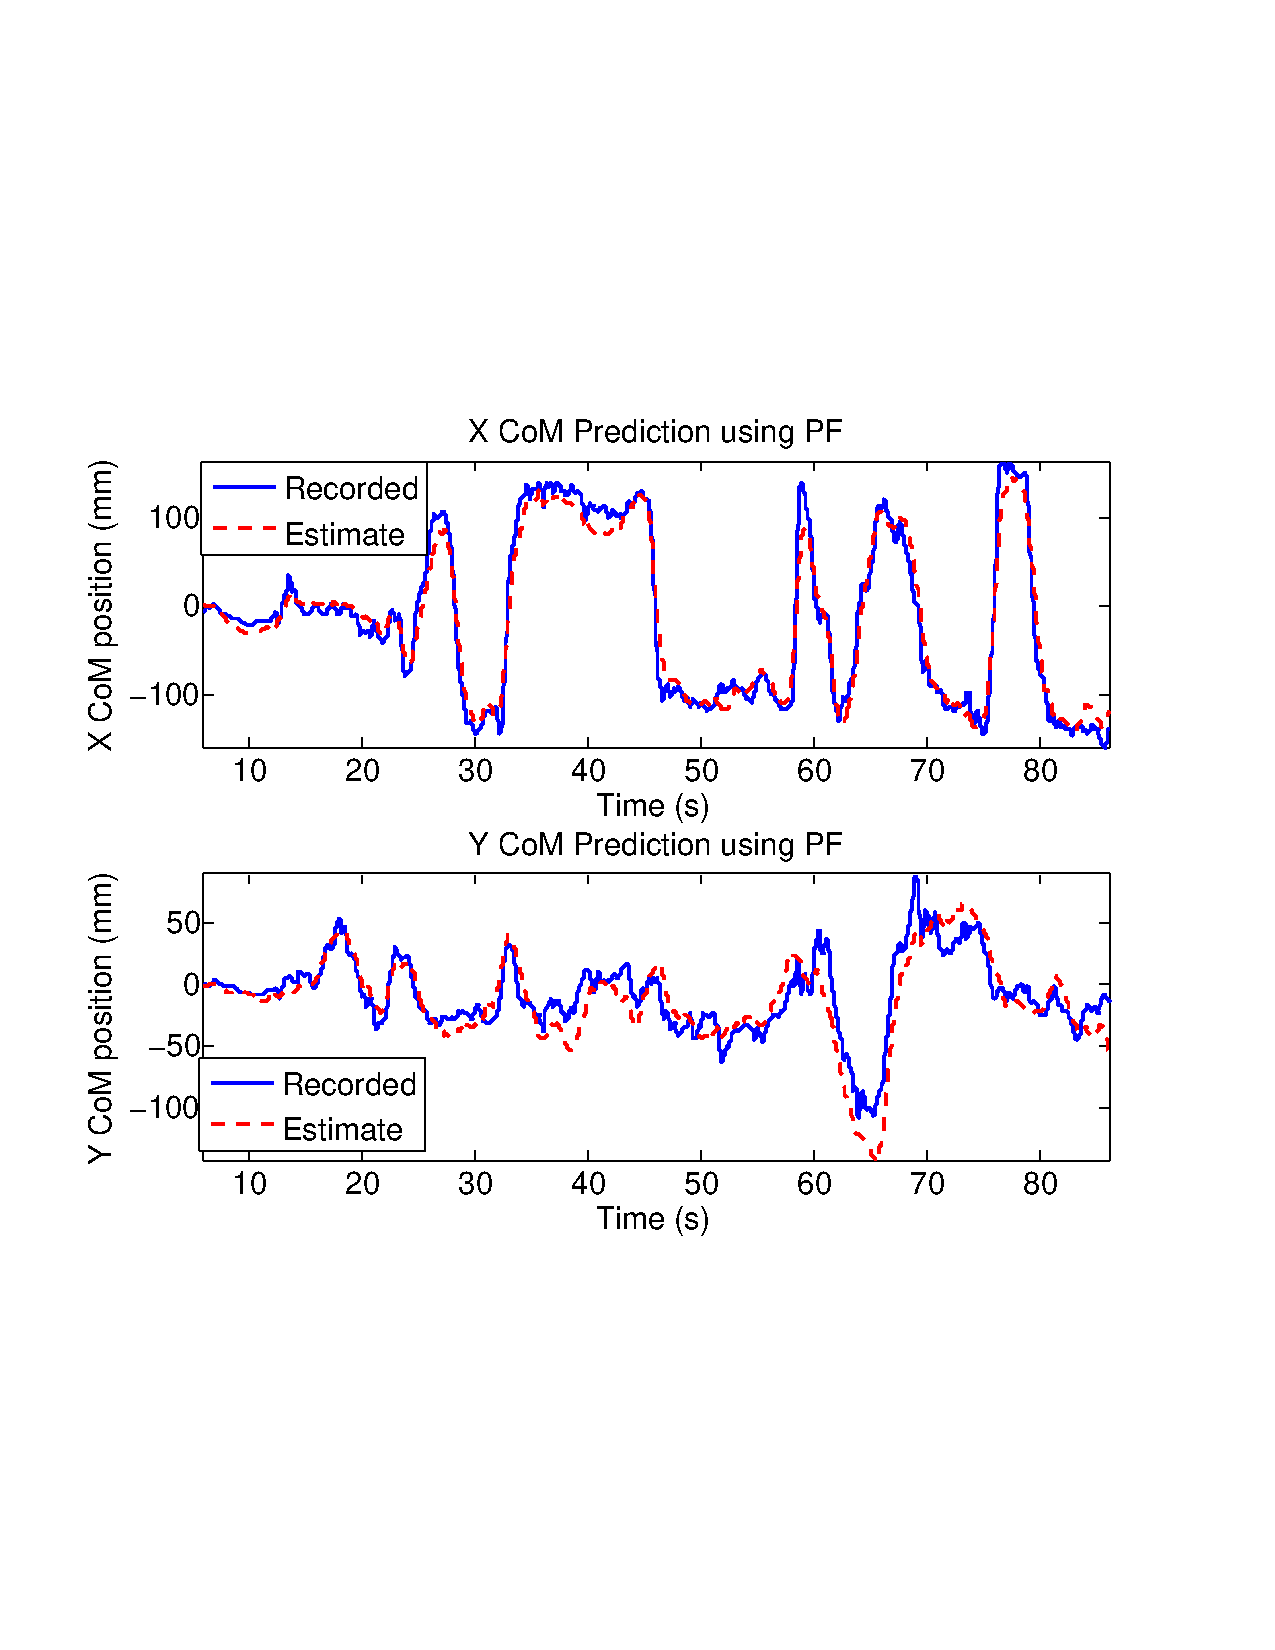
\includegraphics[trim=1cm 6cm 2cm 4cm, clip=true, width=0.9\columnwidth]{figures/PF_Test2.pdf}
%\vspace{-0.15in}
%\caption{CoM prediction using mass distribution obtained by PF }
%\label{fig:com1}
%%\vspace{-0.2in}
%\end{figure}
%
%\begin{figure}
%  \centering
%    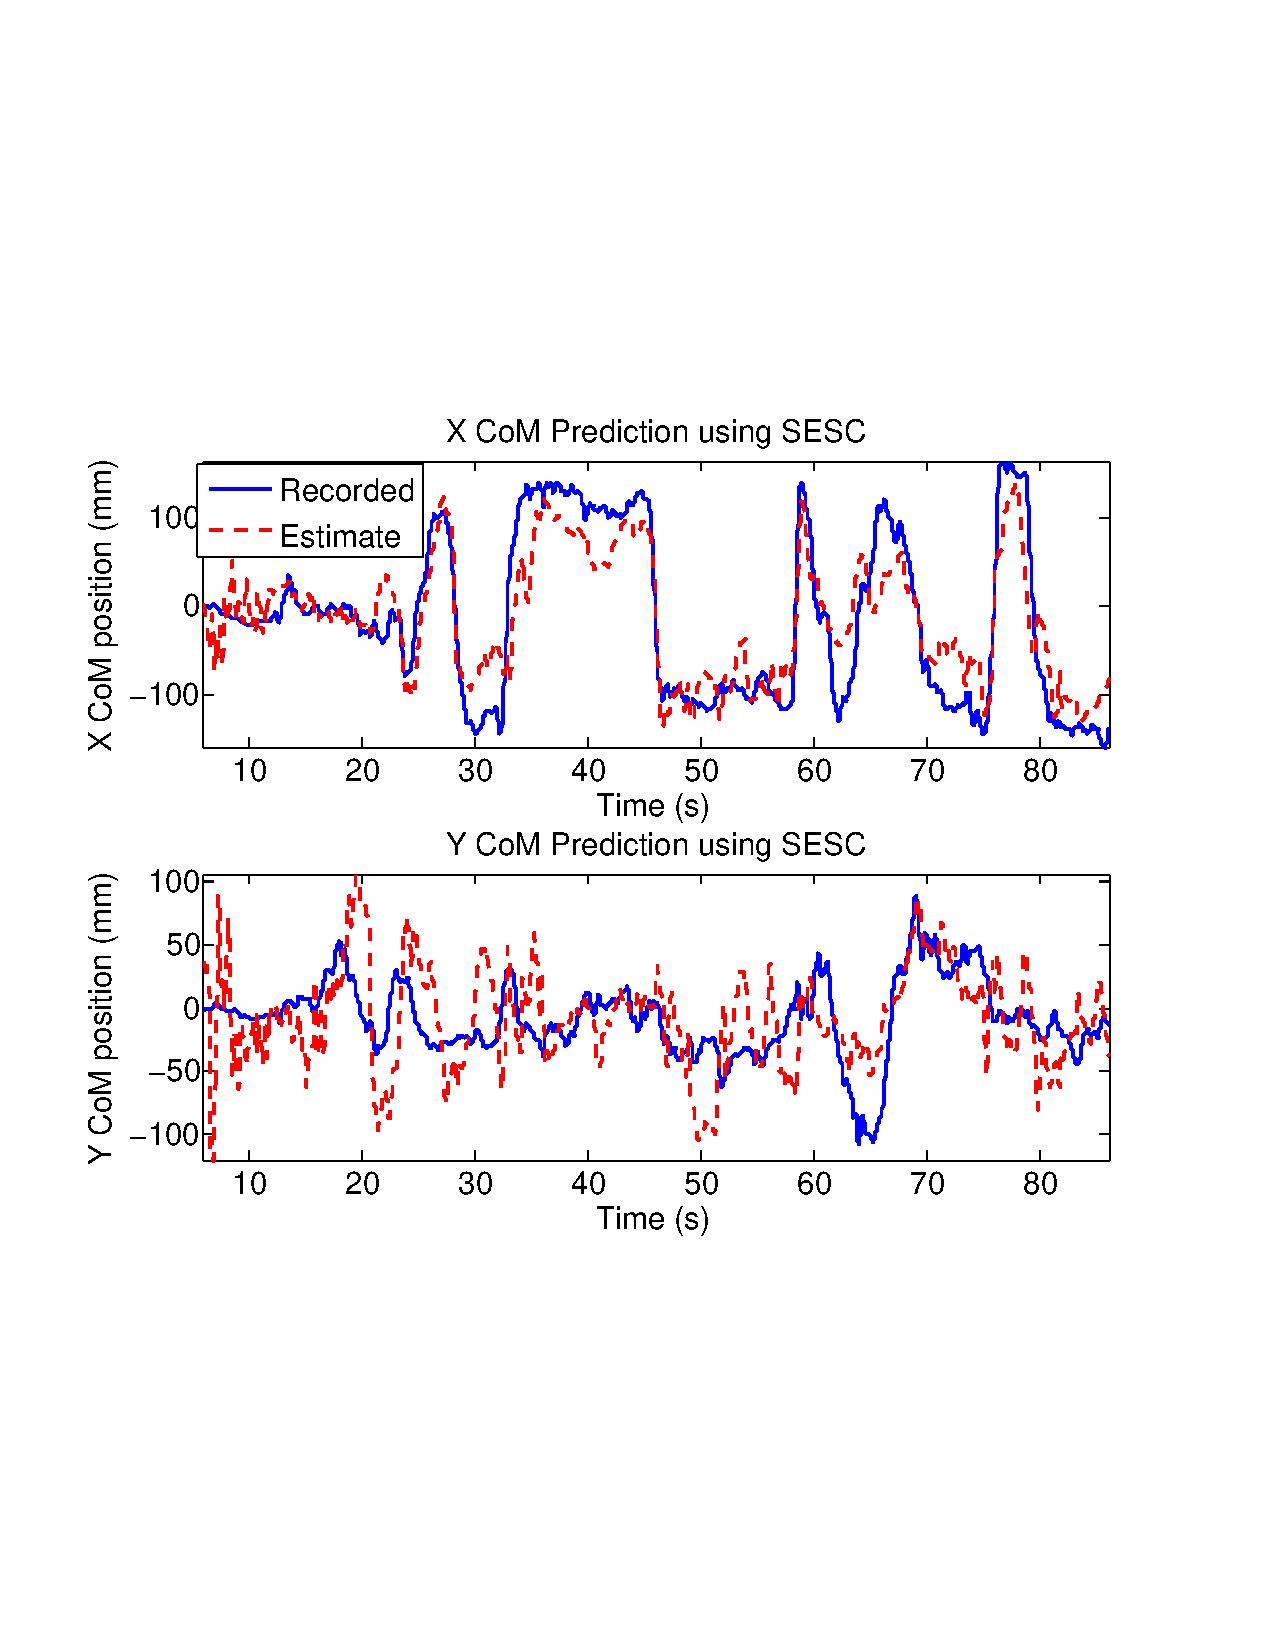
\includegraphics[trim=1cm 6cm 2cm 4cm, clip=true, width=0.9\columnwidth]{figures/SESC_Test2.pdf}
%\vspace{-0.15in}
%\caption{CoM prediction using SESC model}
%\label{fig:com1}
%%\vspace{-0.2in}
%\end{figure}
%
%
%\begin{figure}
%  \centering
%    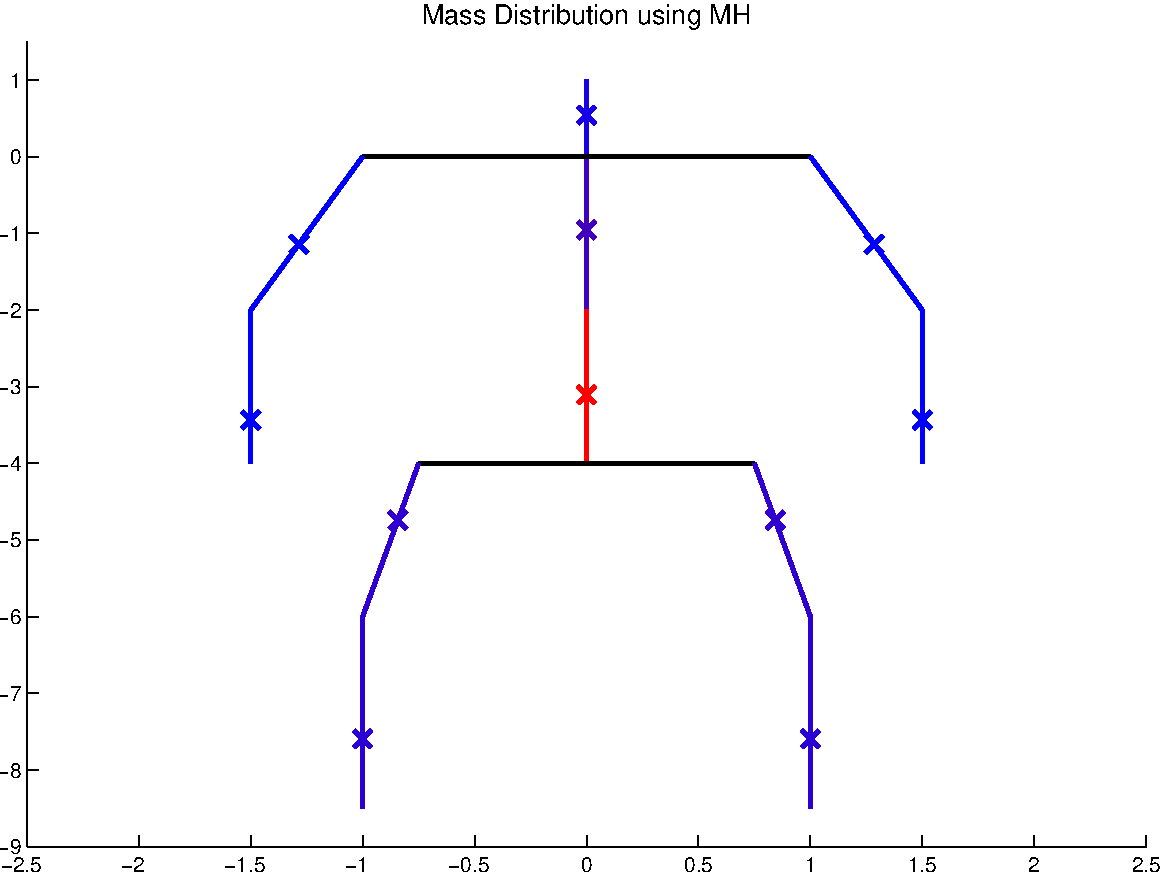
\includegraphics[width=0.85\columnwidth]{figures/Massdist_MH.pdf}
%\vspace{-0.15in}
%\caption{Mass Distribution obtained by MH }%Due to the large state space, changepoint detection and model reclassification is occassionally delayed. }
%\label{fig:com1}
%%\vspace{-0.2in}
%\end{figure}
%
%\begin{figure}
%  \centering
%    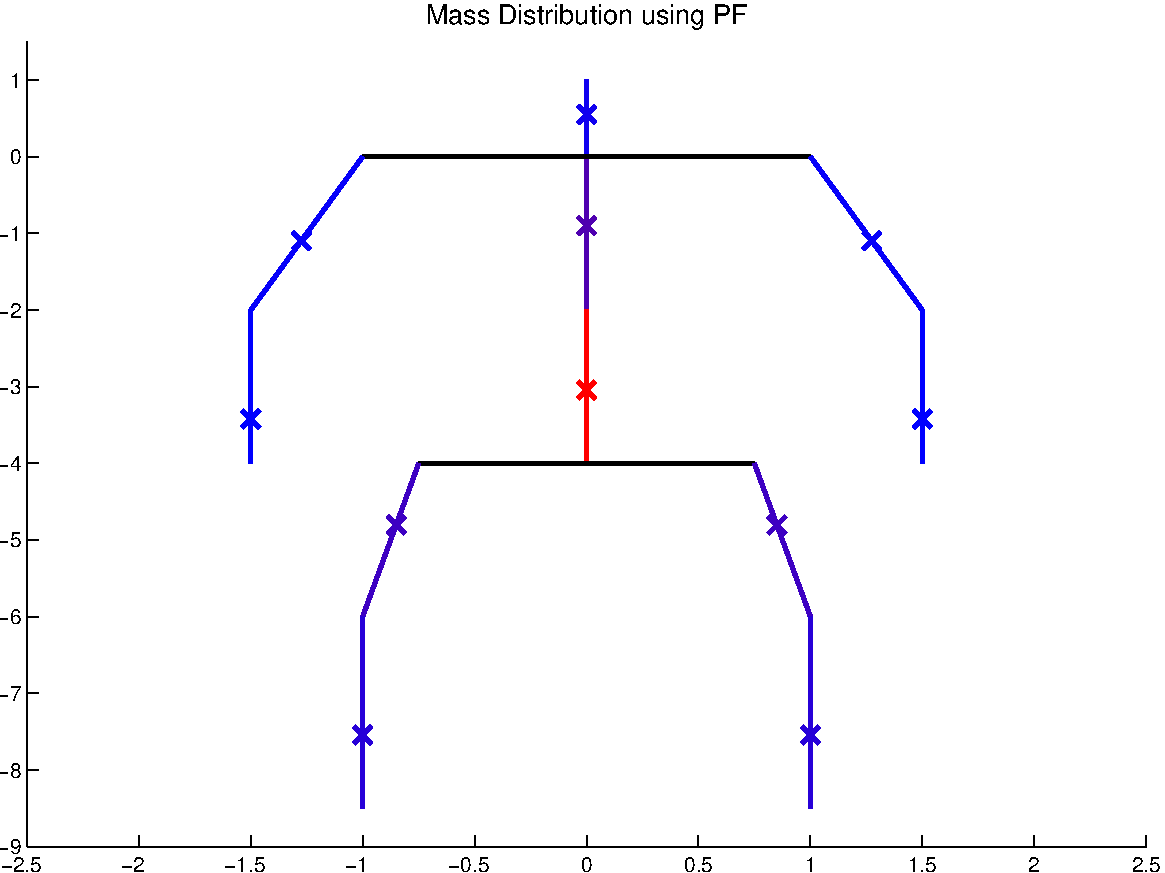
\includegraphics[width=0.85\columnwidth]{figures/Massdist_PF.pdf}
%\vspace{-0.15in}
%\caption{Mass Distribution obtained by PF}%Due to the large state space, changepoint detection and model reclassification is occassionally delayed. }
%\label{fig:com1}
%%\vspace{-0.2in}
%\end{figure}
%
%\begin{figure}
%  \centering
%    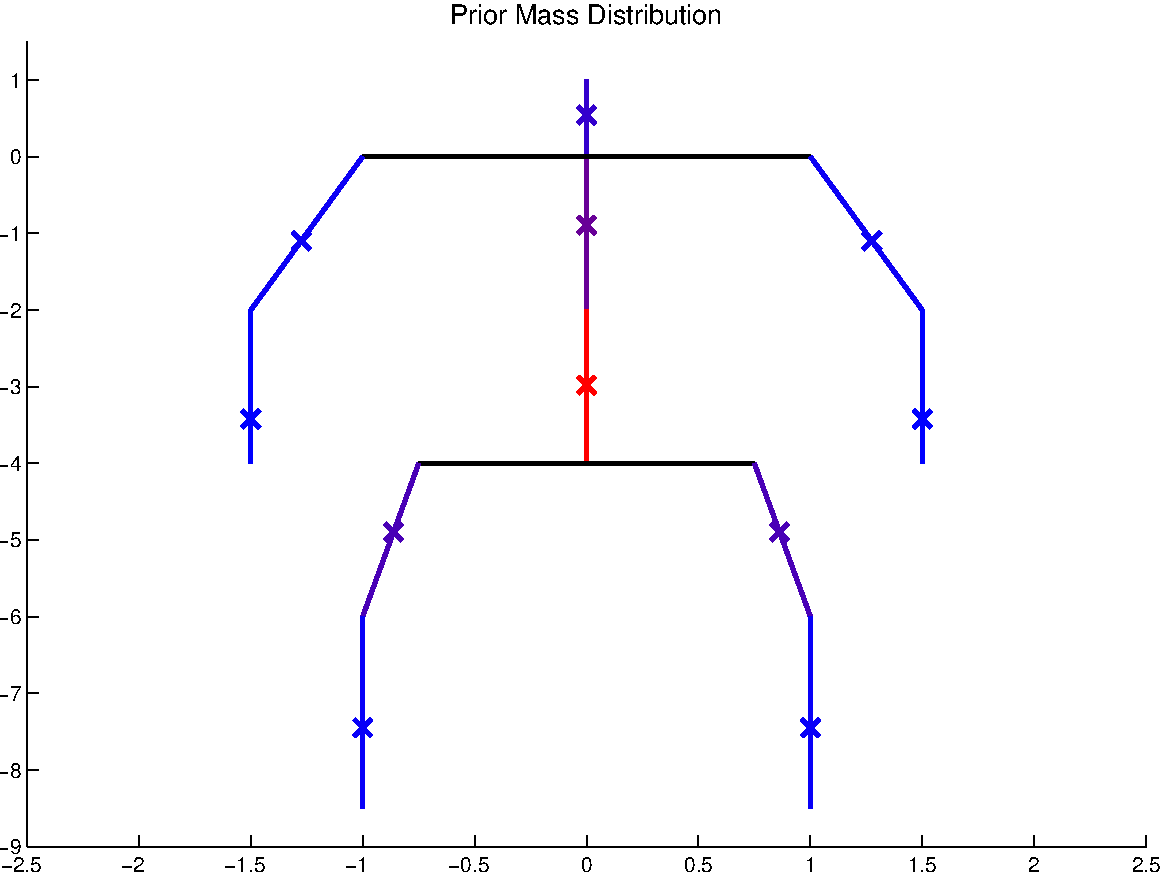
\includegraphics[width=0.85\columnwidth]{figures/Massdist_Prior.pdf}
%\vspace{-0.15in}
%\caption{Prior Mass Distribution}%Due to the large state space, changepoint detection and model reclassification is occassionally delayed. }
%\label{fig:com1}
%%\vspace{-0.2in}
%\end{figure}
%

In general, both the the PF and MH algorithms perform well in terms of predicting the CoM location. Both algorithms outperform the SESC algorithm by approximately a factor a two for all subjects. CoM predictions are generally within 30~mm of the Wii Balance Board prediction, so the prediction capability is quite reliable. On the other hand, the SESC algorithm appears to overfit the parameters and perform poorly, especially in the $y$ dimension. All algorithms had more difficulty in predicting the $y$ position of the CoM, most likely due to the fact that the Kinect sensor is not as accurate in measuring depth. 

The MH and PF algorithms return reasonable estimate for the inertial parameters, although there is some variability between the results returned by the algorithms. It is likely that a more thorough training phase is needed in which the subject performs a greater variety of movements focusing on specific limbs. For example, if a subject lifts his full arm up, the algorithm cannot distinguish the difference between the lower arm and the upper arm, because both are moving simultaneously. On the other hand, if one moves only the lower arm, keeping the upper arm fixed, this would help the algorithm find the true parameters. 

